\documentclass[12pt]{article}

\usepackage{graphicx}
\usepackage{float}
\usepackage{caption}
\usepackage{amsmath}
\renewcommand\refname{Bibliografia} 
\addtolength{\skip\footins}{8pt}
\setlength\intextsep{18pt}
\renewcommand*\contentsname{Indice}
\usepackage{hyperref}
\hypersetup{
    colorlinks,
    citecolor=black,
    filecolor=black,
    linkcolor=black,
    urlcolor=black
}
	
\begin{document}


\begin{titlepage}
  \begin{center}
    
\includegraphics[scale=0.1]{img/logo-unipd.png}\\

    \vspace{0.8cm}
    \textsc{\LARGE Universit\`{a} degli Studi di Padova}\\
    \vspace{0.45cm}
    \textsc{\large Dipartimento di Ingegneria Industriale}\\
    \vspace{0.4cm}
    \textsc{\large Corso di Laurea in}\\
    \textsc{\large Ingegneria Aerospaziale}\\
    \vspace{1.2cm}
    \textsc{\large Tesi di Laurea}\\
    \vfill
    % Title
    { \LARGE \bfseries Raccolta e analisi dei dati di volo per un velivolo a controllo remoto
    }\\
    \vfill
    \textit{\large Relatore:} \hfill \textit{\large Laureando:}\\
    \textsc{\large Prof. Francesco Picano} \hfill \textsc{Emanuele Cason}\\
    \hfill \textsc{1219779}\\

    \vfill
    {\large Anno Accademico 2022/2023}
  \end{center}
\end{titlepage}

\newpage
\tableofcontents
\newpage

\section{Introduzione} 
Nell'ambito del progetto LiftUp del Dipartimento di Ingegneria Industriale, per la partecipazione all'Air Cargo Challenge 2022, è stato progettato e costruito un velivolo a controllo remoto, candidato poi dal nostro team alla competizione.
Tutto il processo di progettazione e realizzazione del drone, si è basato sul regolamento di gara, e in particolare sui requisiti di sistema e sui criteri di attribuzione del punteggio. Di tali criteri, la porzione più rilevante è stata dedicata dalla giuria alle prestazioni in volo dell'aeromobile \cite{regulation}. 
\\\\
Ne è nata la necessità di disporre di un sistema di registrazione e trasmissione dei dati di volo dei sensori, con molteplici importanti finalità, tra cui: 

\begin{itemize}
\item Prevedere i punteggi conseguenti alle singole esercitazioni di preparazione svolte nei mesi precedenti alla gara.
\item Individuare le migliori condizioni di manovra.
\item Verificare l'accettabilità delle approssimazioni, delle relazioni analitiche e dei processi adottati durante il dimensionamento e design preliminare del velivolo.
\item Valutare le prestazioni durante il collaudo.
\end{itemize}

\noindent
A seguito di varie valutazioni sulla possibilità di acquistare sistemi di telemetria già pronti all'uso, si è optato per progettare, sviluppare e integrare un modulo specifico da zero, al fine di avere maggiore controllo sulle caratteristiche, migliore consapevolezza del suo funzionamento e maggiore margine di intervento (ad esempio reiterandone il design per ridurne la massa, ottimizzando la trasmissione e la visualizzazione dei dati, \textit{eccetera}) in base alle necessità emergenti, anche nell'ottica di disporre di un sistema comodo da implementare nei velivoli che verranno sviluppati in futuro.
\\\\
Anche in termini di costi tale scelta risulta molto vantaggiosa: un sistema pre-fabbricato infatti richiede l'acquisto di sensori e componenti aggiuntivi compatibili, spesso limitando la scelta ad un marchio unico e con protocolli non open-source. Al contrario, nel sistema progettato è stato possibile considerare un trade-off per ogni componente e sensore, scegliendo quello più conveniente in termini di prezzo e prestazioni, anche affidandosi a produttori diversi. 

\section{Struttura del sistema di telemetria}
In linea generale, il sistema è stato articolato in due nodi. Uno installato a bordo del velivolo e l'altro complementare, parte di una stazione di terra.

\subsection{Dispositivo lato velivolo}
Il dispositivo a bordo del velivolo è stato progettato con un architettura centralizzata, programmato con un firmware appositamente creato. Il microcontrollore, nello specifico Arduino Nano, interroga tutti i sensori installati e per mezzo di un modulo dotato di slot micro-SD ne memorizza i valori in un file creato appositamente sulla scheda inserita. Simultaneamente, gli stessi dati vengono trasmessi a terra per mezzo di un componente rice-trasmettitore alla frequenza di 2.4 GHz. Lo stesso componente, riceve eventuali comandi (ad esempio per avviare la registrazione dei dati, o per calibrare la IMU) dalla stazione di terra, e li inoltra al microcontrollore perché vengano eseguiti.

\begin{figure}[h]
	\centering
	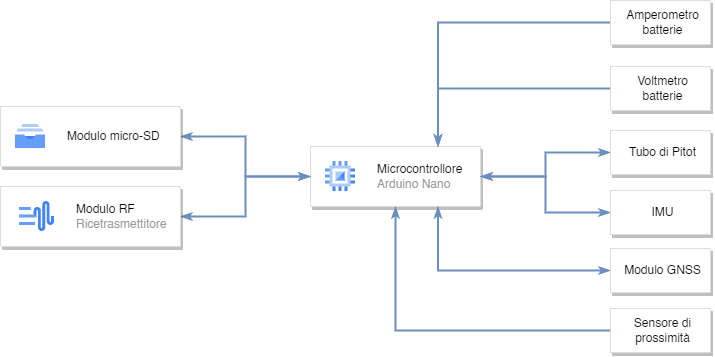
\includegraphics[width=13cm]{img/RADAR-Arch}
\end{figure}

\noindent
Un altra caratteristica del sistema, derivante dall'architettura scelta è la sua modularità. L'intero sistema infatti, può essere rapidamente adattato per raccogliere e trasmettere a terra i dati di un insieme variabile di sensori connessi. Questo aspetto ha avuto particolare utilità nelle prime fasi del collaudo, durante le quali, viste le scadenze ravvicinate, è stato necessario implementare rapidamente una prima versione del sistema di telemetria, anche a patto di disporre dei dati di un numero ridotto di sensori connessi.

\begin{figure}[!h]
	\centering
	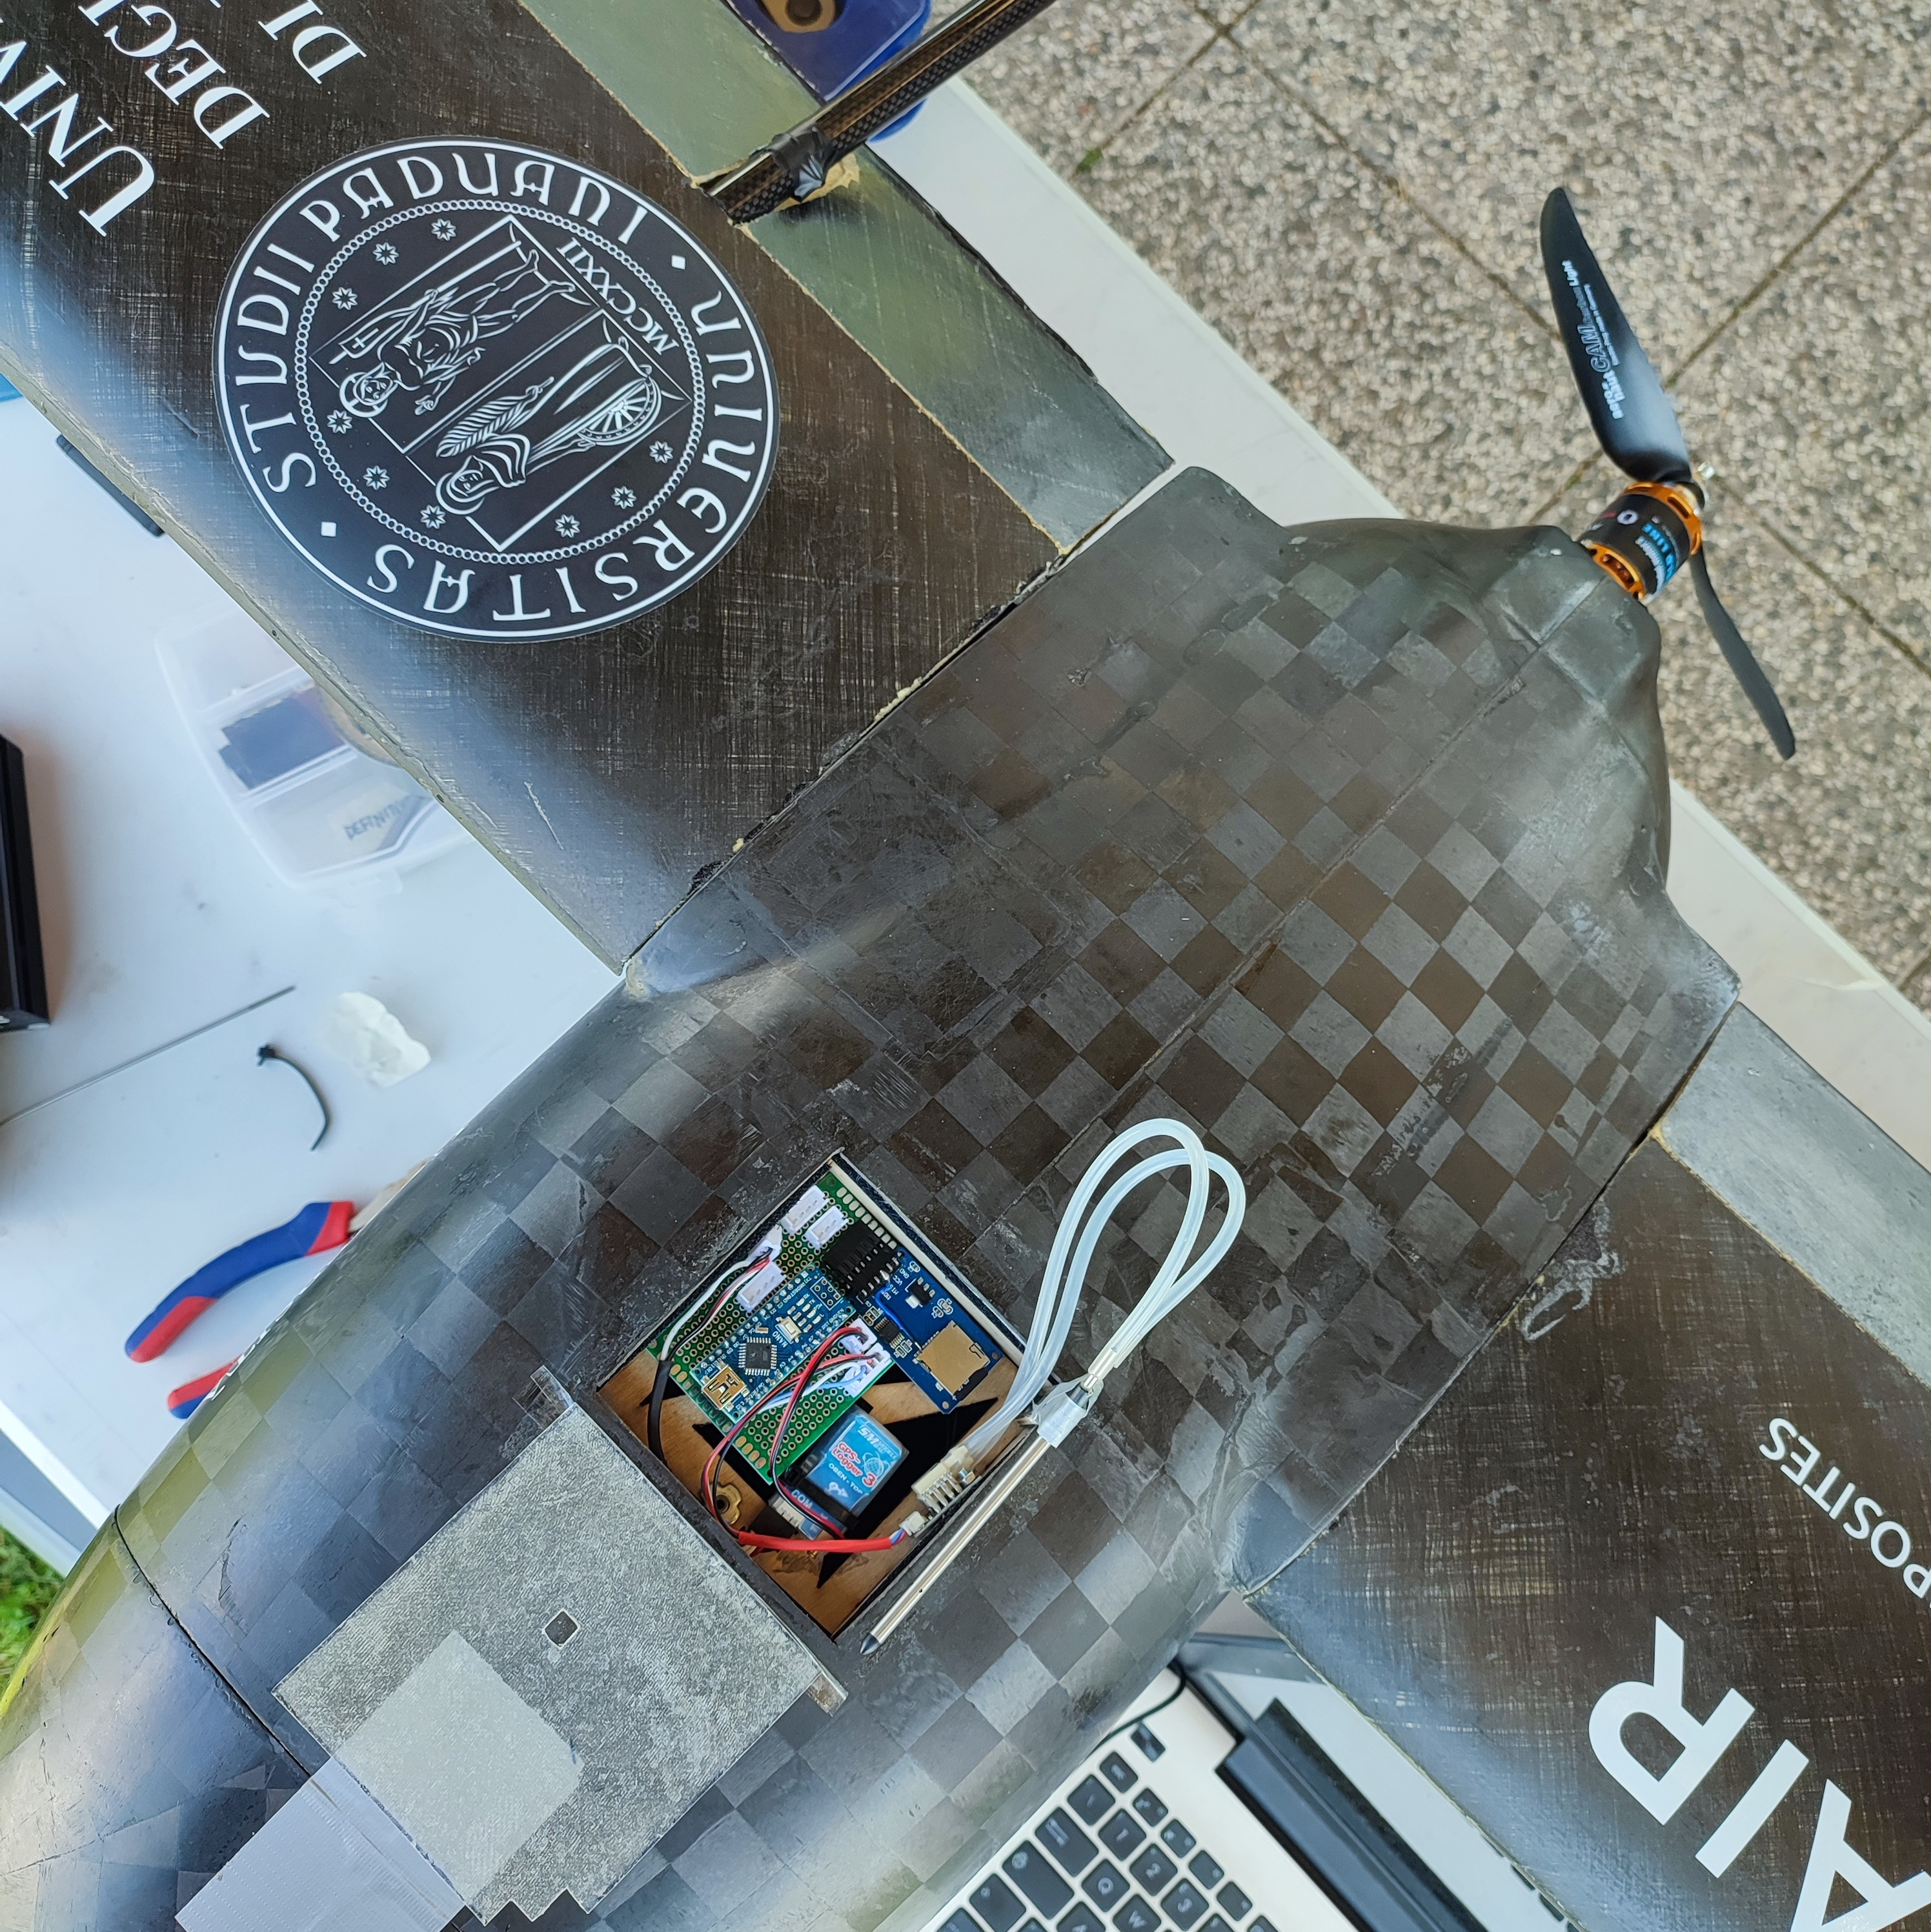
\includegraphics[width=6.5cm]{img/ph-radar}
	\,
	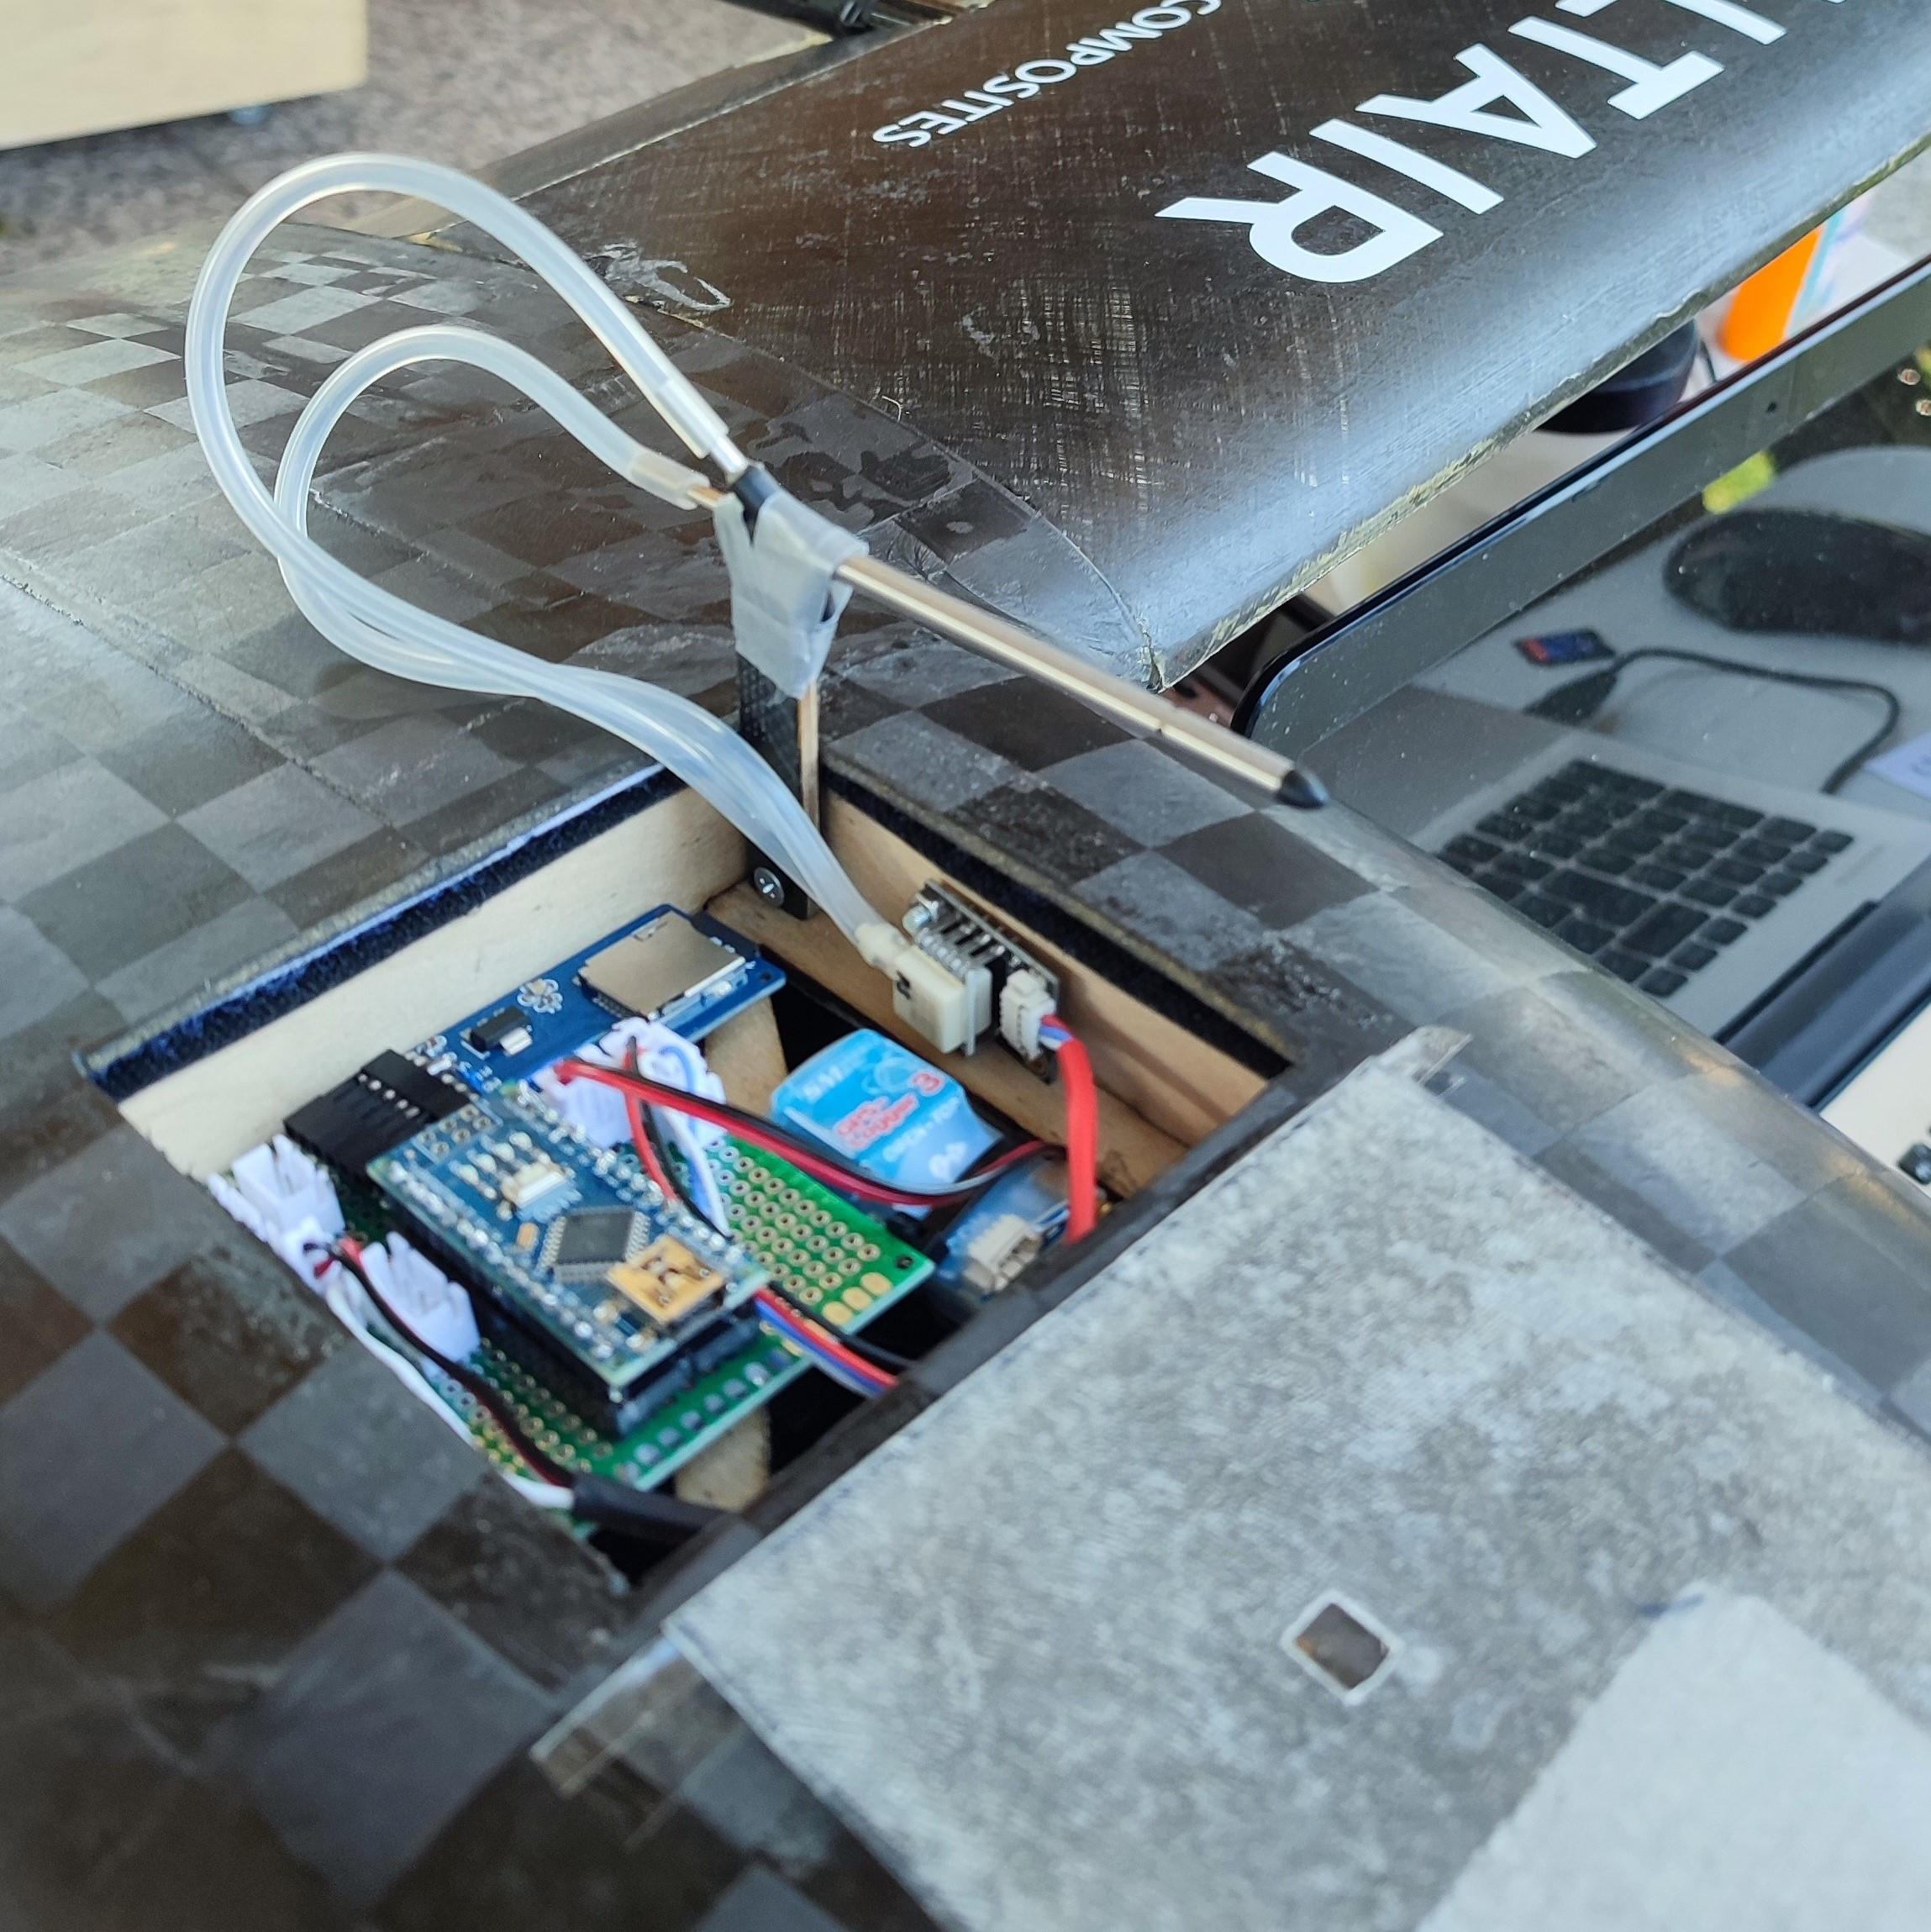
\includegraphics[width=6.5cm]{img/ph-radar-near}
	\captionsetup{labelformat=empty}
\end{figure}

\begin{figure}[!h]
	\centering
	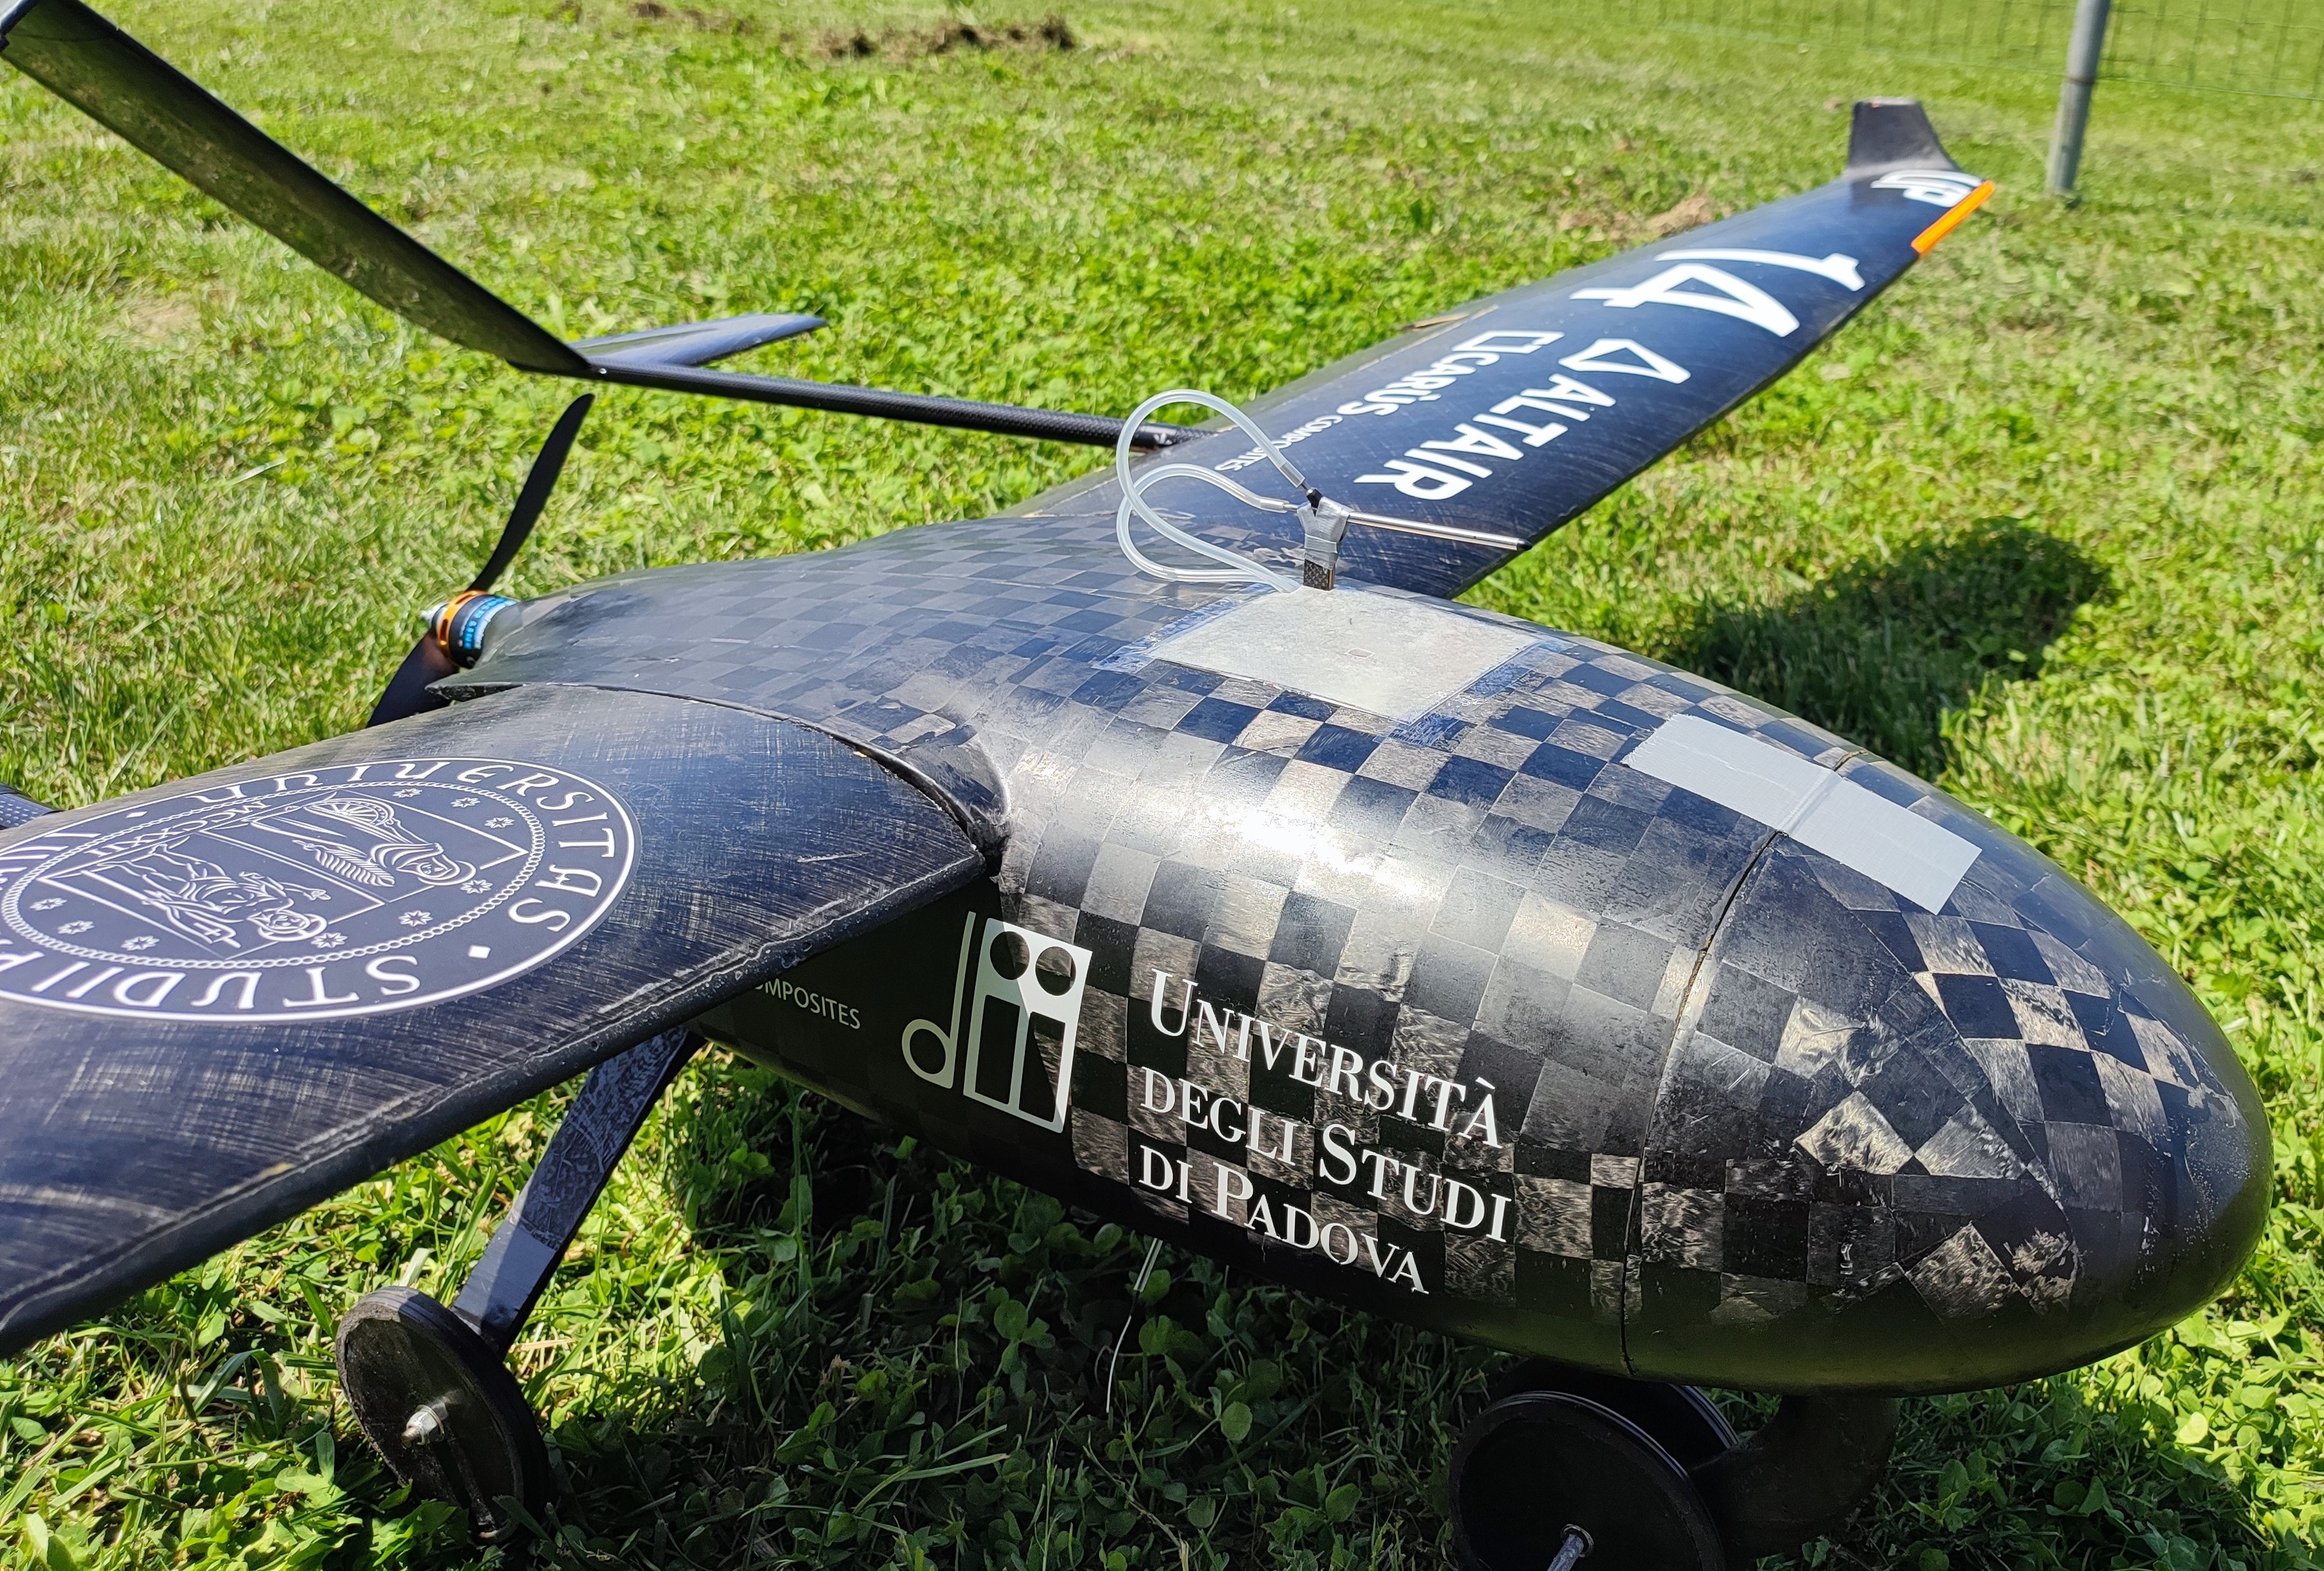
\includegraphics[width=13.35cm]{img/ph-radar-closed}
	\captionsetup{labelformat=empty}
\end{figure}


\subsubsection{Modulo GNSS}
Il modulo ricevitore GNSS \footnote{"Global Navigation Satellite System", termine generico per indicare sistemi di cui fanno parte GPS, GLONASS, GALILEO, ecc. In seguito per semplicità si utilizzeranno equivalentemente gli acronimi GPS e GNSS.} è stato scelto in base a vari fattori considerati: in primis la consistenza dei dati con quelli che sarebbero stati raccolti in competizione (dove da regolamento la giuria utilizza lo stesso modulo per calcolare i punteggi di gara), i valori di risoluzione e velocità di aggiornamento dei dati relativamente alti, la compatibilità con i sistemi a bordo dell'aeromodello e di radiocontrollo, e non ultimo il costo non eccessivamente alto. Il modulo integra inoltre accelerometro a tre assi e barometro, consente la registrazione dei dati su una scheda microSD indipendente da quella principale e il loro invio simultaneo a dispositivi che supportano il protocollo FrSky Smart Port, per la telemetria in tempo reale.
\\\\
Se da un lato scegliere lo stesso modulo utilizzato dalla giuria è stato vantaggioso in termini di coerenza e affidabilità dei dati raccolti, l'implementazione della trasmissione in diretta dei dati a terra ha causato non poche complicazioni. Si è reso necessario infatti decodificare il protocollo proprietario Smart Port per renderlo leggibile dal microcontrollore, per mezzo di una libreria appositamente riadattata, operazione fortemente complicata dalla scarsità della documentazione resa pubblica sul funzionamento del protocollo.

\subsubsection{Modulo rice-trasmettitore}
A seguito di svariati test condotti su alcuni moduli acquistati negli anni precedenti, operanti a 433 Mhz, sono saltati subito all'occhio problemi come latenze di trasmissione troppo elevate, bassi data rate, portate insufficienti.
La scelta di moduli più performanti per la trasmissione a terra dei dati (e l'eventuale ricezione di comandi inerenti alla telemetria), si è basata su vari requisiti, tra cui: la compatibilità con la tensione di alimentazione disponibile e consumo elettrico accettabile; un protocollo di comunicazione con il microcontrollore semplice da implementare; l'utilizzo di segnale a modulazione digitale; data rate e portata  sufficientemente elevati; e la presenza di un connettore coassiale per l'antenna, in modo da localizzarla all'esterno della fusoliera in fibra di carbonio, per evitare il suo effetto radio-attenuante.
\\\\
Una volta individuato il dispositivo, è stato possibile effettuare una verifica teorica della sua portata, a partire dai valori indicati nel datasheet \cite{rf-datasheet}. Considerando, in ottica conservativa, la potenza minima di trasmissione e la potenza minima in ricezione, per mantenere il data rate a $250 \textnormal{ kbps}$:
\begin{equation}
\begin{split}
P_{tx} &= 19.7 \textnormal{ dBm} = 0.0933 \textnormal{ W} \\
P_{rx} &= -96 \textnormal{ dBm} = 2.51 \cdot 10^{-13} \textnormal{ W}
\end{split}
\end{equation}

\noindent
Nota l'equazione della trasmissione di Friis, nell'ipotesi di antenne isotrope in trasmissione e ricezione (ovvero con guadagno $G = 0 \textnormal{ dBi} = 1$), trascurando perdite diverse da quella spaziale di propagazione (come perdite di linea, di interferenza, atmosferiche, eccetera):
\begin{equation}
P_{rx} = P_{tx} \cdot G_{tx} \cdot G_{rx} \cdot \left(\frac{\lambda}{4 \pi D}\right)^2
\end{equation}
Si ottiene una portata massima teorica $D = 6060 \textnormal{ m}$. Essendo tale valore non inferiore alla portata richiesta (dell'ordine di 2000 m), è risultato sensato procedere all'acquisto e al successivo test sperimentale che, pur registrando distanze ben inferiori a quella teorica (intorno a 2300 m), probabilmente dovute alle perdite trascurate, ha confermato la sufficienza della distanza raggiunta.

\subsection{Stazione di terra}
La stazione di terra permette il monitoraggio in tempo reale dei valori misurati dai sensori. Per mezzo di un modulo di rice-trasmettitore complementare a quello precedentemente descritto e connesso ad un altro microcontrollore, vengono ricevuti e decodificati i pacchetti provenienti dal velivolo e i relativi dati inviati al computer tramite comunicazione seriale. 

\begin{figure}[h]
	\centering
	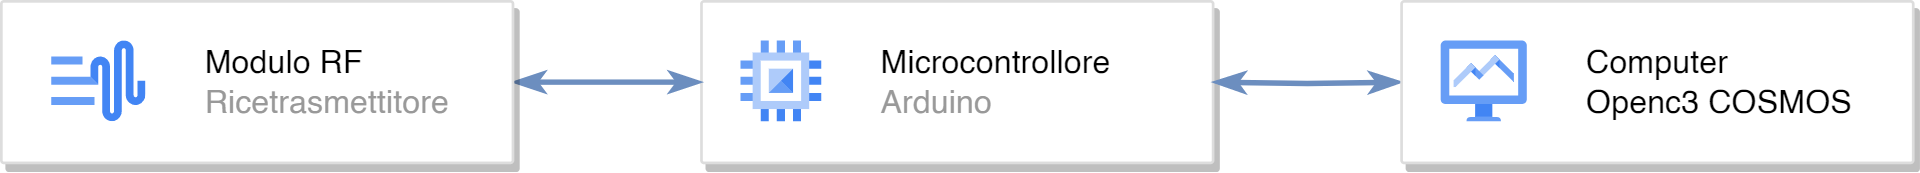
\includegraphics[width=13cm]{img/GS-Arch}
\end{figure}

\noindent 
Il software che è stato scelto per il monitoraggio, la visualizzazione e il plot dei dati in tempo reale, è OpenC3 COSMOS, software gratuito e open-source, inizialmente sviluppato da Ball Aerospace e utilizzato in svariate missioni spaziali incluse GMI, OLI, Kepler, WISE, OMPS, Ares, Orion, e numerosi programmi di difesa \cite{cosmos}. Dato da riportare a proposito di tale software è la sua contro intuitività nella fase di configurazione, che va effettuata scrivendo manualmente file testuali di setup, secondo una documentazione che pur essendo molto ben curata va a trascurare molti particolari non sempre sottintesi. Nonostante questo svantaggio tuttavia, le potenzialità offerte hanno reso comunque conveniente il suo impiego.

\section{Previsione dei punteggi}
Già dai primi voli di collaudo, al fine di ottenere un resoconto quantitativo sui punteggi che i medesimi voli avrebbero totalizzato se fossero stati eseguiti in gara, si è reso necessario disporre dei dati di posizione. In questa circostanza di urgenza dovuta alle scadenze ravvicinate, si è sfruttata la modularità del sistema, implementando il solo modulo GNSS e momentaneamente rinunciando alla restante sensoristica. Il sistema ha così permesso di registrare i dati di localizzazione del velivolo e di riceverli a terra in diretta. A seguito di ogni volo, per mezzo di un programma appositamente sviluppato in Python, è stato svolto il post-processing dei file di log, per ricavare i dati utili.
\\\\
I tre fattori principali per l'attribuzione del punteggio del singolo volo, come da regolamento \cite{regulation}, sono stati:
\begin{itemize}
\item \textbf{Payload} trasportato durante il volo, misurato in termini di massa.
\item \textbf{Altitudine} raggiunta a 60 secondi del tempo di volo.
\item \textbf{Distanza} coperta tra il secondo 60 e il secondo 180 del tempo di volo.
\end{itemize}
Dove l'inizio della misura del tempo di volo è stato definito in corrispondenza del raggiungimento di 5 km/h di velocità rispetto al suolo (misurata dal modulo GNSS), durante la fase di decollo.
\\\\
Una criticità inizialmente riscontrata ha riguardato la rilevazione dell'istante di decollo. Si sono infatti osservati, soprattutto nelle fasi immediatamente precedenti a quest'ultimo, picchi di velocità non ragionevoli. A seguito di varie ipotesi si è concluso che tali imprecisioni dei dati erano originate dal cold start del ricevitore GNSS. L'iniziale imprecisione dei dati durante la fase di fixing dei satelliti infatti, ha talvolta falsato le letture di posizione, e di conseguenza le velocità rispetto al suolo derivate, causando falsi decolli e quindi errori di calcolo dei parametri di output. 
\\\\
Per ovviare al problema, si è proceduto su due fronti. Sono stati implementati in primo luogo un comando da terra di inizio registrazione in modo tale da avviare la registrazione dopo il fix di un numero sufficiente di satelliti, e in secondo luogo un approccio grafico nel post-processing, tale da permettere di validare l'istante di decollo effettivo rilevato in automatico, sulla base dei dati di velocità ed altitudine visualizzati in un diagramma, al fine di accertare la validità dei dati in seguito prodotti. 
\\\\
Nell'immagine sottostante ad esempio è ben visibile come il plot dei dati permetta di distinguere un falso positivo del decollo (evidenziato in rosso), dal decollo effettivo, garantendo il corretto ottenimento dei dati di output (a sinistra).

\begin{figure}[!h]
	\centering
	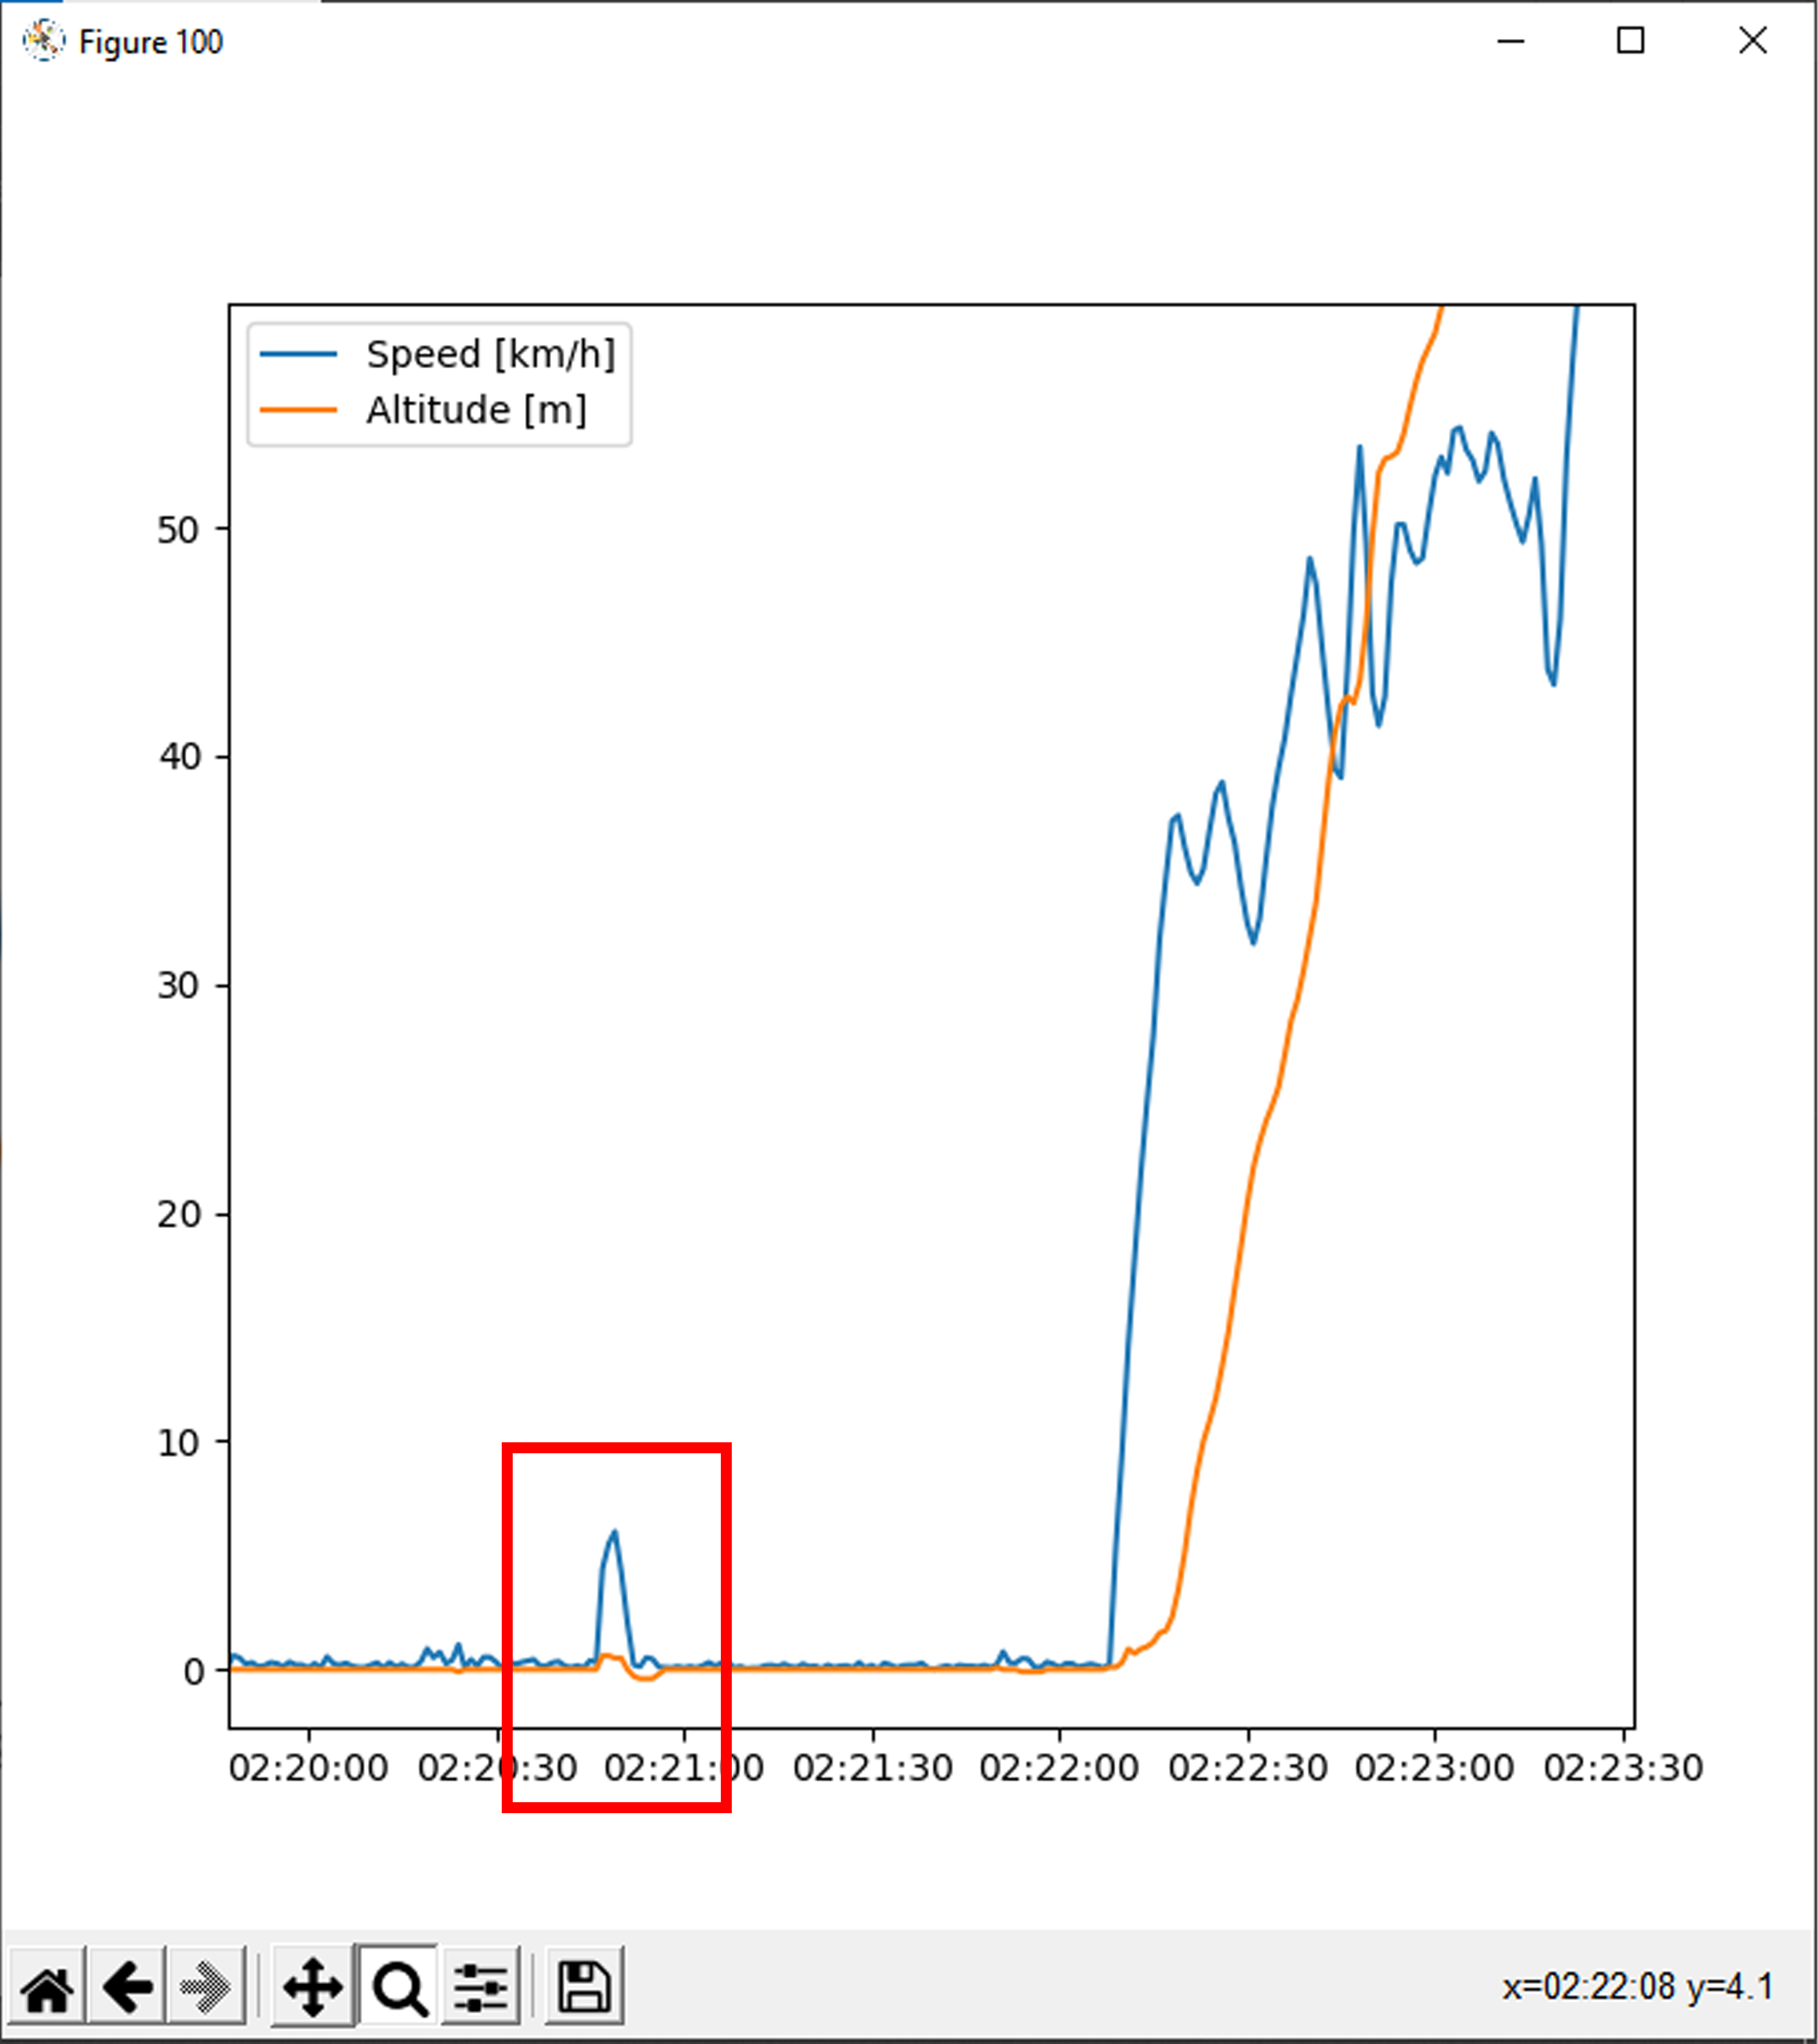
\includegraphics[width=6.5cm]{img/diagramma-decollo}
	\quad
	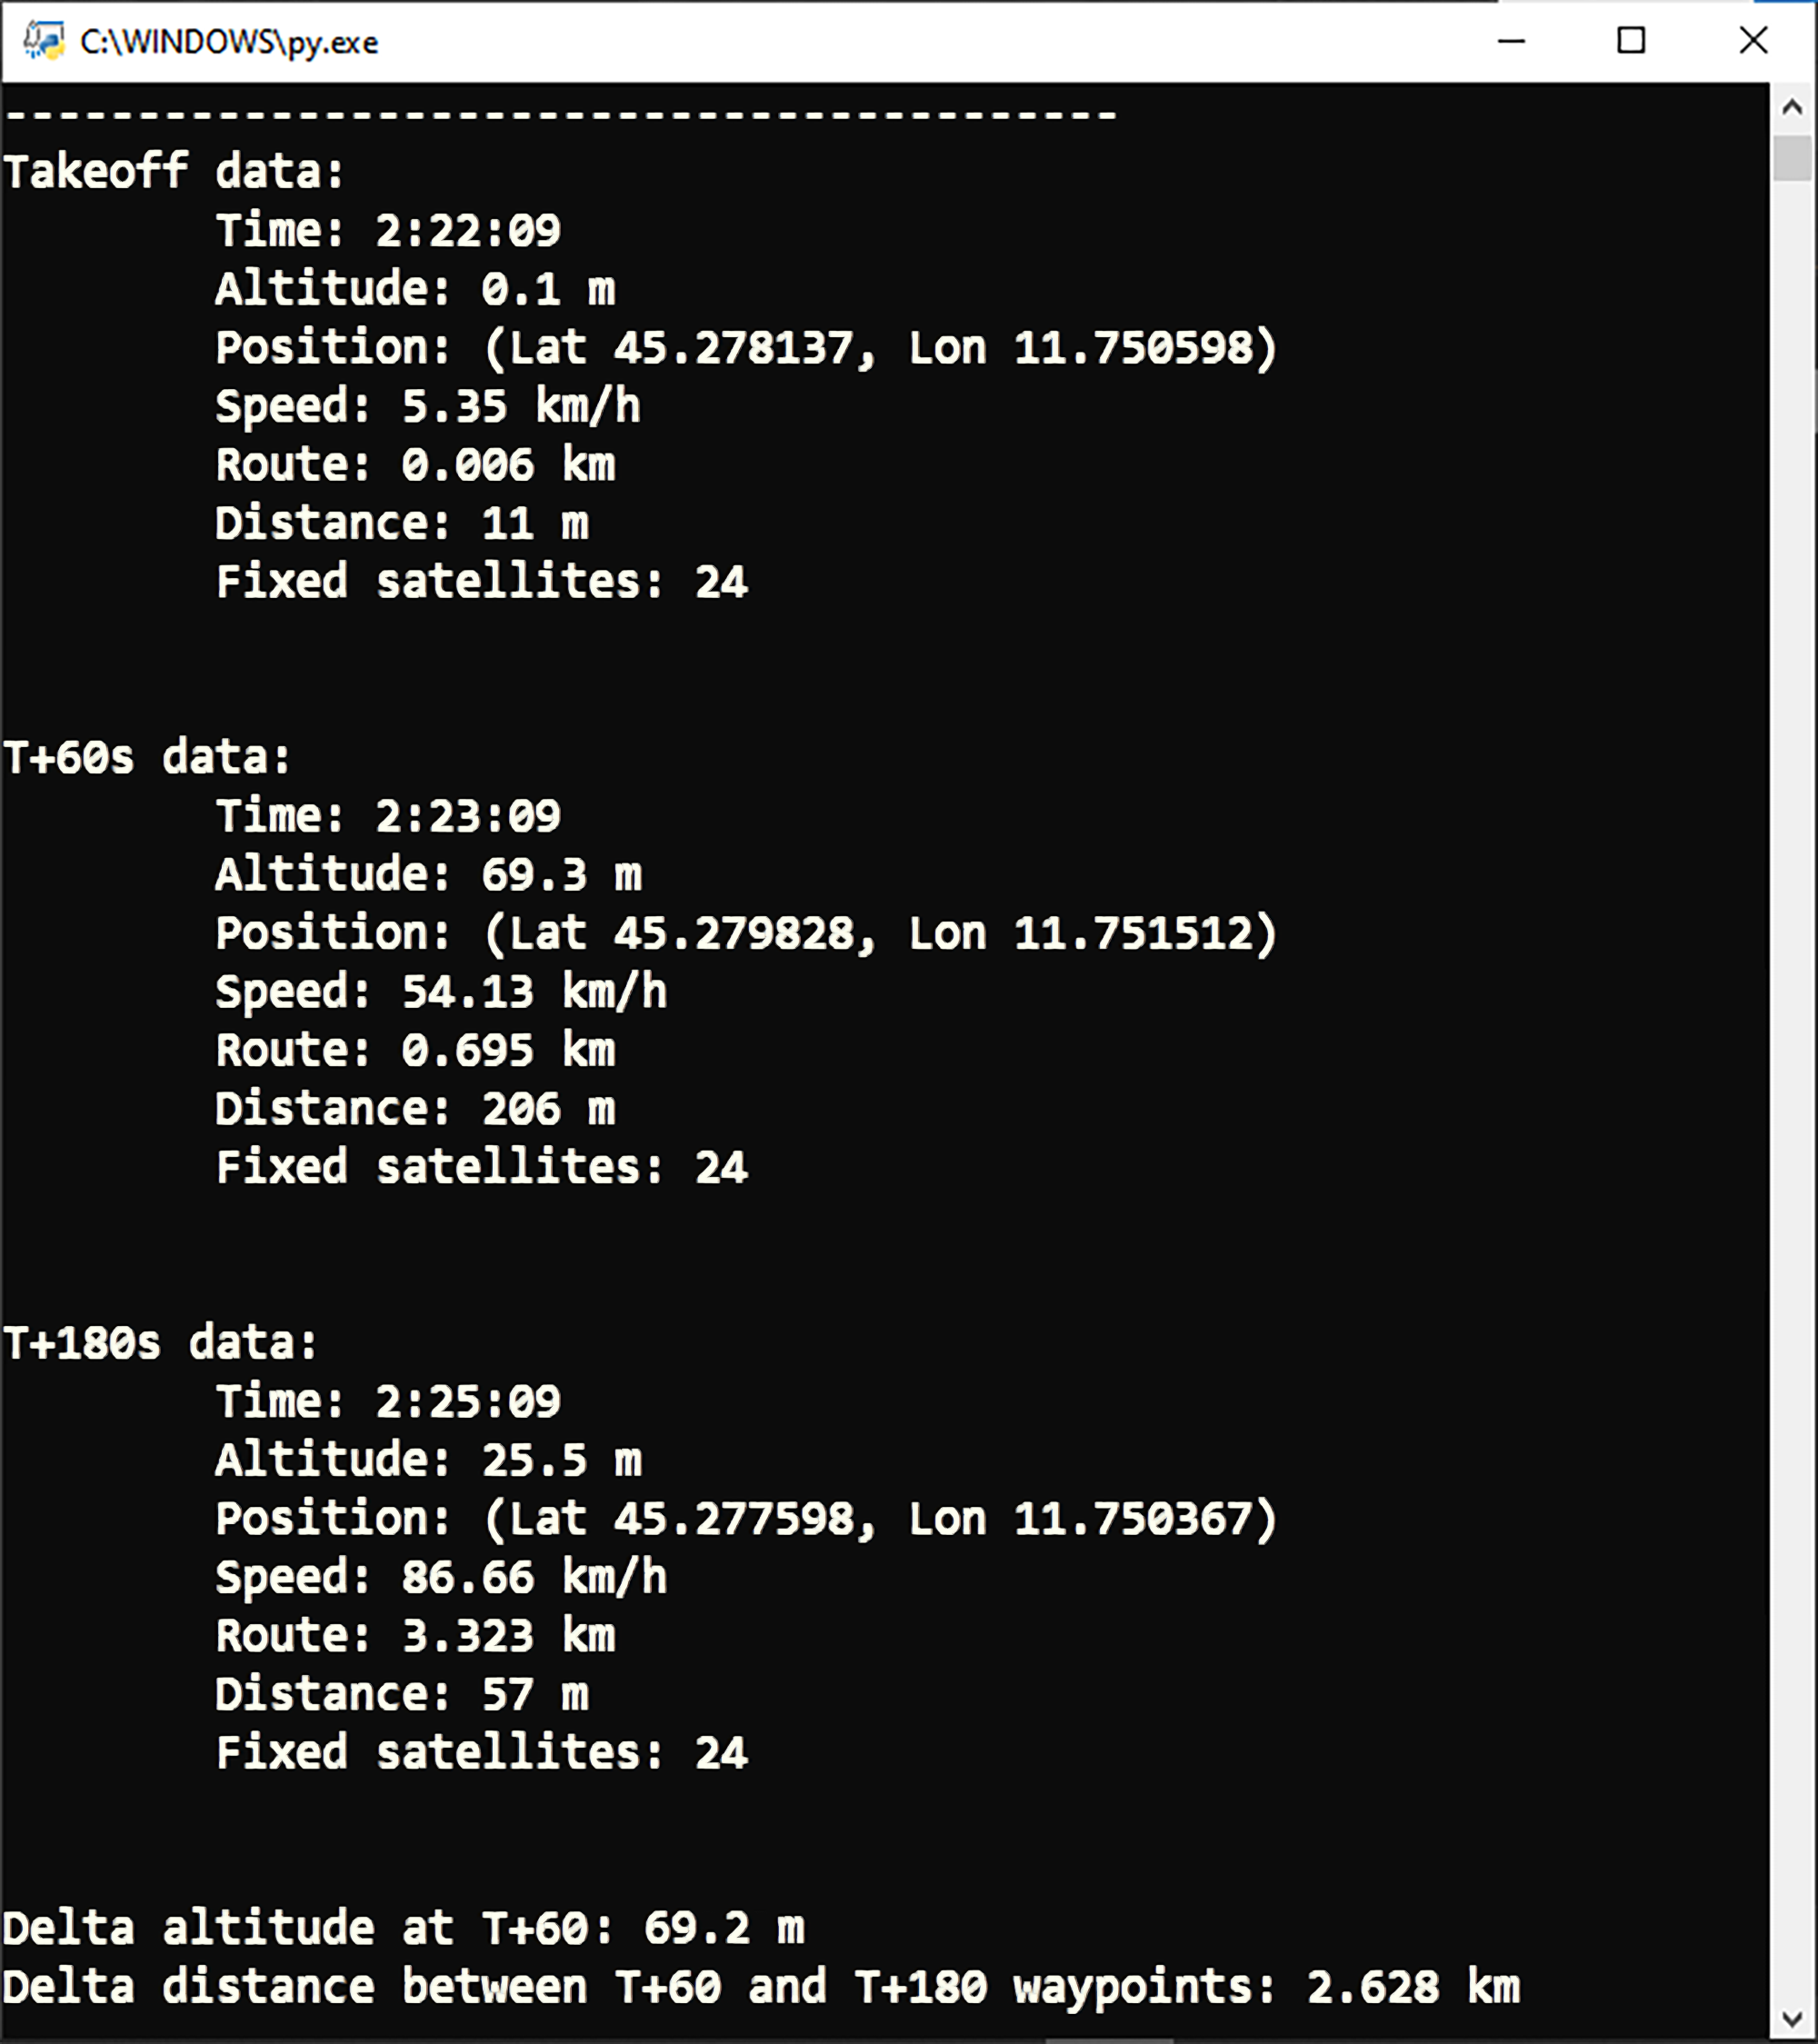
\includegraphics[width=6.5cm]{img/screenshot}
	\captionsetup{labelformat=empty}
	\caption{Volo 3 - 6 marzo 2022, ore 14:22:09}
\end{figure}

\section{Verifica del processo di dimensionamento del velivolo}
Il processo di dimensionamento e progettazione preliminare del velivolo, rappresenta una fase fondamentale per l'ottenimento di un aereo con buone prestazioni. Allo stesso tempo però, il fatto di partire da zero, con un grande numero di requisiti e grandezze obbiettivo da considerare, rende questa operazione altamente complessa, a tal punto che lo stesso algoritmo di dimensionamento si potrebbe considerare un progetto a se stante. 
\\\\
Nel corso degli anni, nonostante il variare dei requisiti imposti dal regolamento, la metodologia per ottenere il progetto preliminare è rimasta molto simile e su di essa è stato fondato il lavoro del team per la progettazione di dettaglio e la manifattura dei velivoli candidati alle ultime edizioni della Air Cargo Challenge del 2019 e 2022.
\\\\
Come spesso accade nell'ambito ingegneristico, soprattutto nello scontrarsi con problemi complessi, l'approssimazione assume importanza cruciale. In modo complementare, la verifica delle approssimazioni impiegate è anch'essa fondamentale, per garantire risultati attendibili. Per questa ragione, con l'implementazione del sistema di telemetria, si ha finalmente la possibilità di verificare puntualmente, per mezzo dei dati empirici raccolti, la validità delle approssimazioni assunte durante il dimensionamento preliminare e quantificare l'impatto degli eventuali errori introdotti, allo scopo di affinare il processo e renderlo più solido.

\subsection{Il processo di dimensionamento in sintesi}
Si riassumono brevemente in seguito i vari passaggi del processo di dimensionamento finora adottati e descritti nei report tecnici definitivi del 2019 \cite{report2019} e del 2022 \cite{report2022}:
\begin{enumerate}
\item In primo luogo viene fissato un set di valori per le variabili di massa totale ($M_{TOT}$), coefficiente di lift massimo ($C_{L, max}$) e distanza di decollo ($X_{TO}$). 
\item Sulla base di questi valori, viene determinata la velocità di decollo ($V_{TO}$), riferita all'istante di liftoff, al quale il velivolo si solleva da terra, ovvero quando forza peso e portanza arrivano ad equivalenza.
\item Nota la velocità di decollo necessaria, viene calcolata la superficie alare richiesta per generare la relativa portanza, e considerati i limiti dimensionali e le condizioni per la stabilità, è ottenuta una geometria di massima del velivolo, in termini di superficie alare e del piano di coda.
\item Per ogni geometria ottenuta a partire dal set di dati iniziali fissato, l'algoritmo calcola le performance di salita e crociera, e sulla base dei criteri del regolamento, i punteggi conseguenti. Il set di dati che massimizza i punteggi è quello che viene scelto, e i relativi $M_{TOT}$, $X_{TO}$ e $C_{L, max}$ diventano i valori obbiettivo per il progetto di dettaglio.
\end{enumerate}
Il flowchart dell'algoritmo assume quindi la struttura seguente:
\begin{figure}[h]
	\centering
	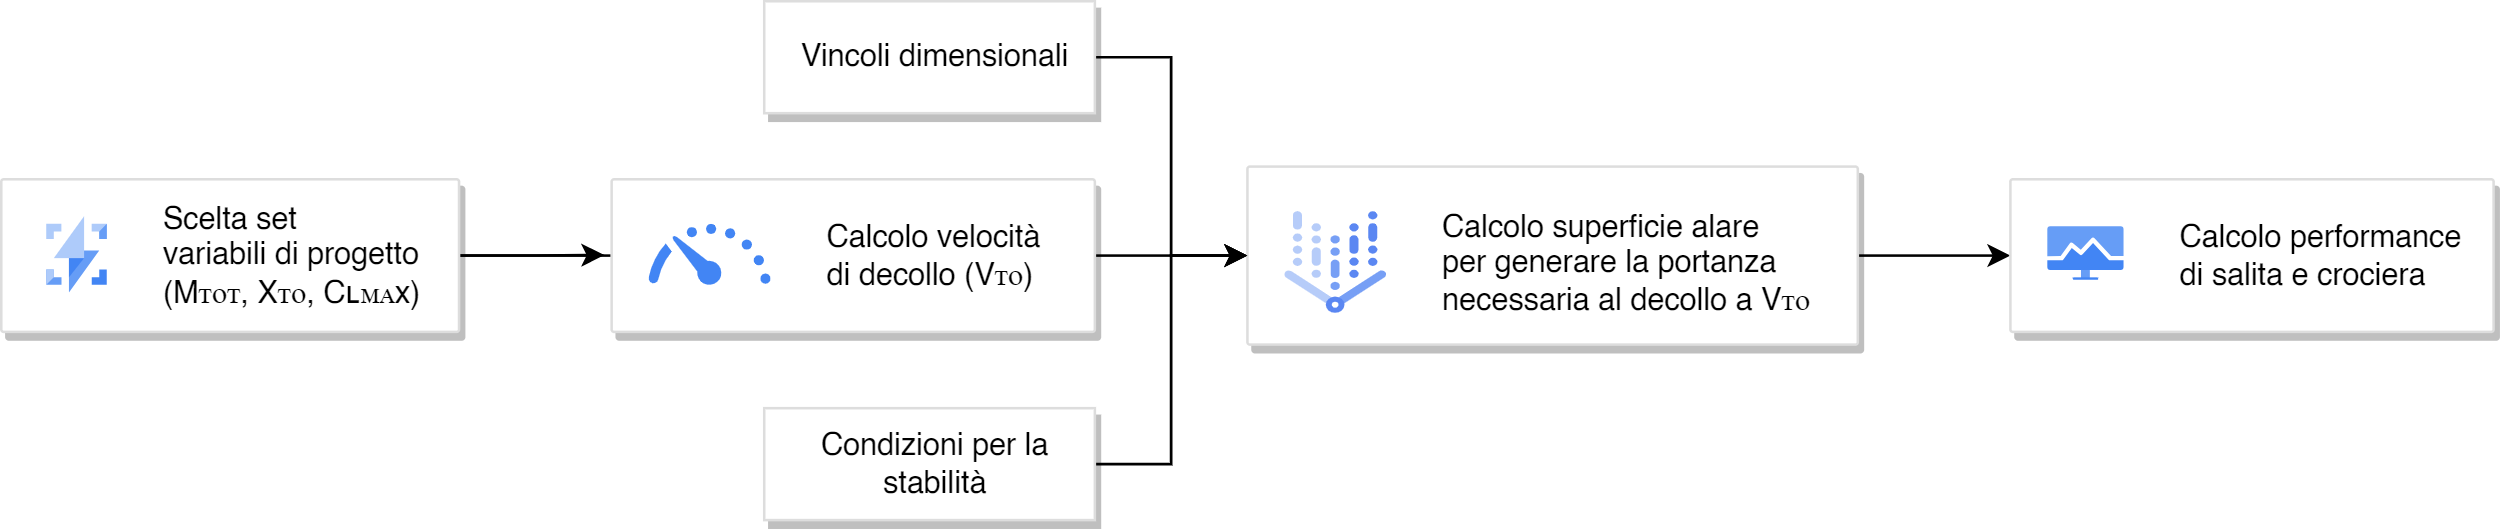
\includegraphics[width=14cm]{img/dimensionamento}
\end{figure}

\subsection{Criticità del secondo step}
A costruzione ultimata, durante il collaudo e la competizione, si è osservata una discrepanza del valore della distanza di decollo di progetto, che era stata imposta a 40 metri, rispetto al quella reale, prevalentemente intorno ai 60 metri, fatto che peraltro ha comportato alcune penalizzazioni in gara. Questo ha spinto a investigare il secondo step del processo, relativo alla stima della velocità di decollo necessaria e critico in quanto in corrispondenza di esso vengono introdotte ipotesi e approssimazioni forti. In particolare: 

\begin{itemize}
\item[2.1] Viene stimata la potenza meccanica erogata all'albero del motore per mezzo del software eCalc, a partire dai dati di batteria, motore, regolatore di velocità, \textit{eccetera}. Tale potenza meccanica viene poi moltiplicata per il rendimento dell'elica, il cui valore, che è funzione della velocità e degli RPM, è fornito dai dati del costruttore. Ipotizzato che al decollo la manetta sia regolata al 100\%, e quindi gli RPM siano costanti, si ottiene la potenza propulsiva disponibile in funzione della velocità ($P_A$).

\item[2.2] Nota la potenza disponibile ($P_A$) e i dati di progetto scelti allo step 1 (in particolare $M_{TOT}$, $X_{TO}$), viene calcolata la velocità di decollo. In questo caso le ipotesi introdotte, da verificare, sono quelle di drag aerodinamico del velivolo e attrito volvente del carrello trascurabili ($D = 0$, $F_{AV} = 0$). 

\begin{figure}[h]
	\centering
	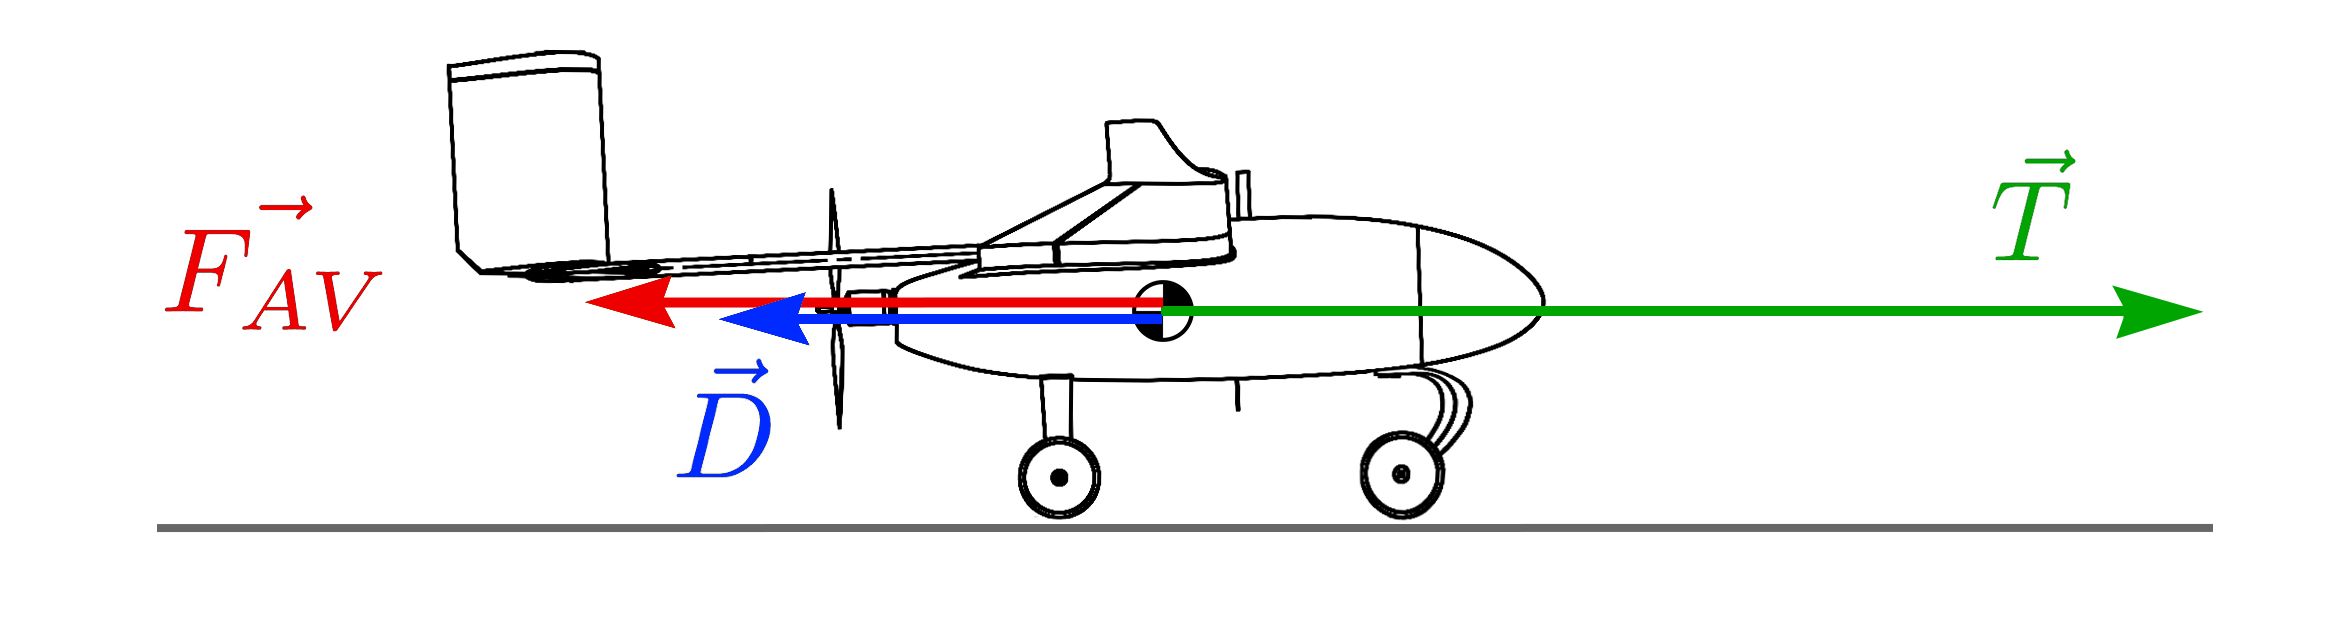
\includegraphics[width=13cm]{img/forze}
\end{figure}

Sotto tali assunzioni, per il secondo principio della dinamica, l'accelerazione orizzontale del velivolo al decollo dipende unicamente dalla forza propulsiva (thrust, $T$), secondo la relazione:

\begin{equation}
T = M_{TOT} \cdot a = M_{TOT} \cdot \frac{dV_\infty}{dt} \cdot \frac{dx}{dx} = M_{TOT} \cdot \frac{V_\infty \cdot dV_\infty}{dx}
\end{equation}

\noindent
Quindi, isolando il termine $dx$ e integrando, si ottiene la velocità al decollo:

\begin{equation}
dx = M_{TOT} \cdot \frac{V_\infty \cdot dV_\infty}{T} \quad \Rightarrow \quad X_{TO} = M_{TOT} \cdot \int_0^{V_{TO}} \, \frac{V_\infty^2}{P_A(v)} \cdot dV_\infty
\end{equation}
\end{itemize}

\noindent
Nel dettaglio quindi, il secondo step ha la struttura descritta dal diagramma sottostante.
\begin{figure}[h]
	\centering
	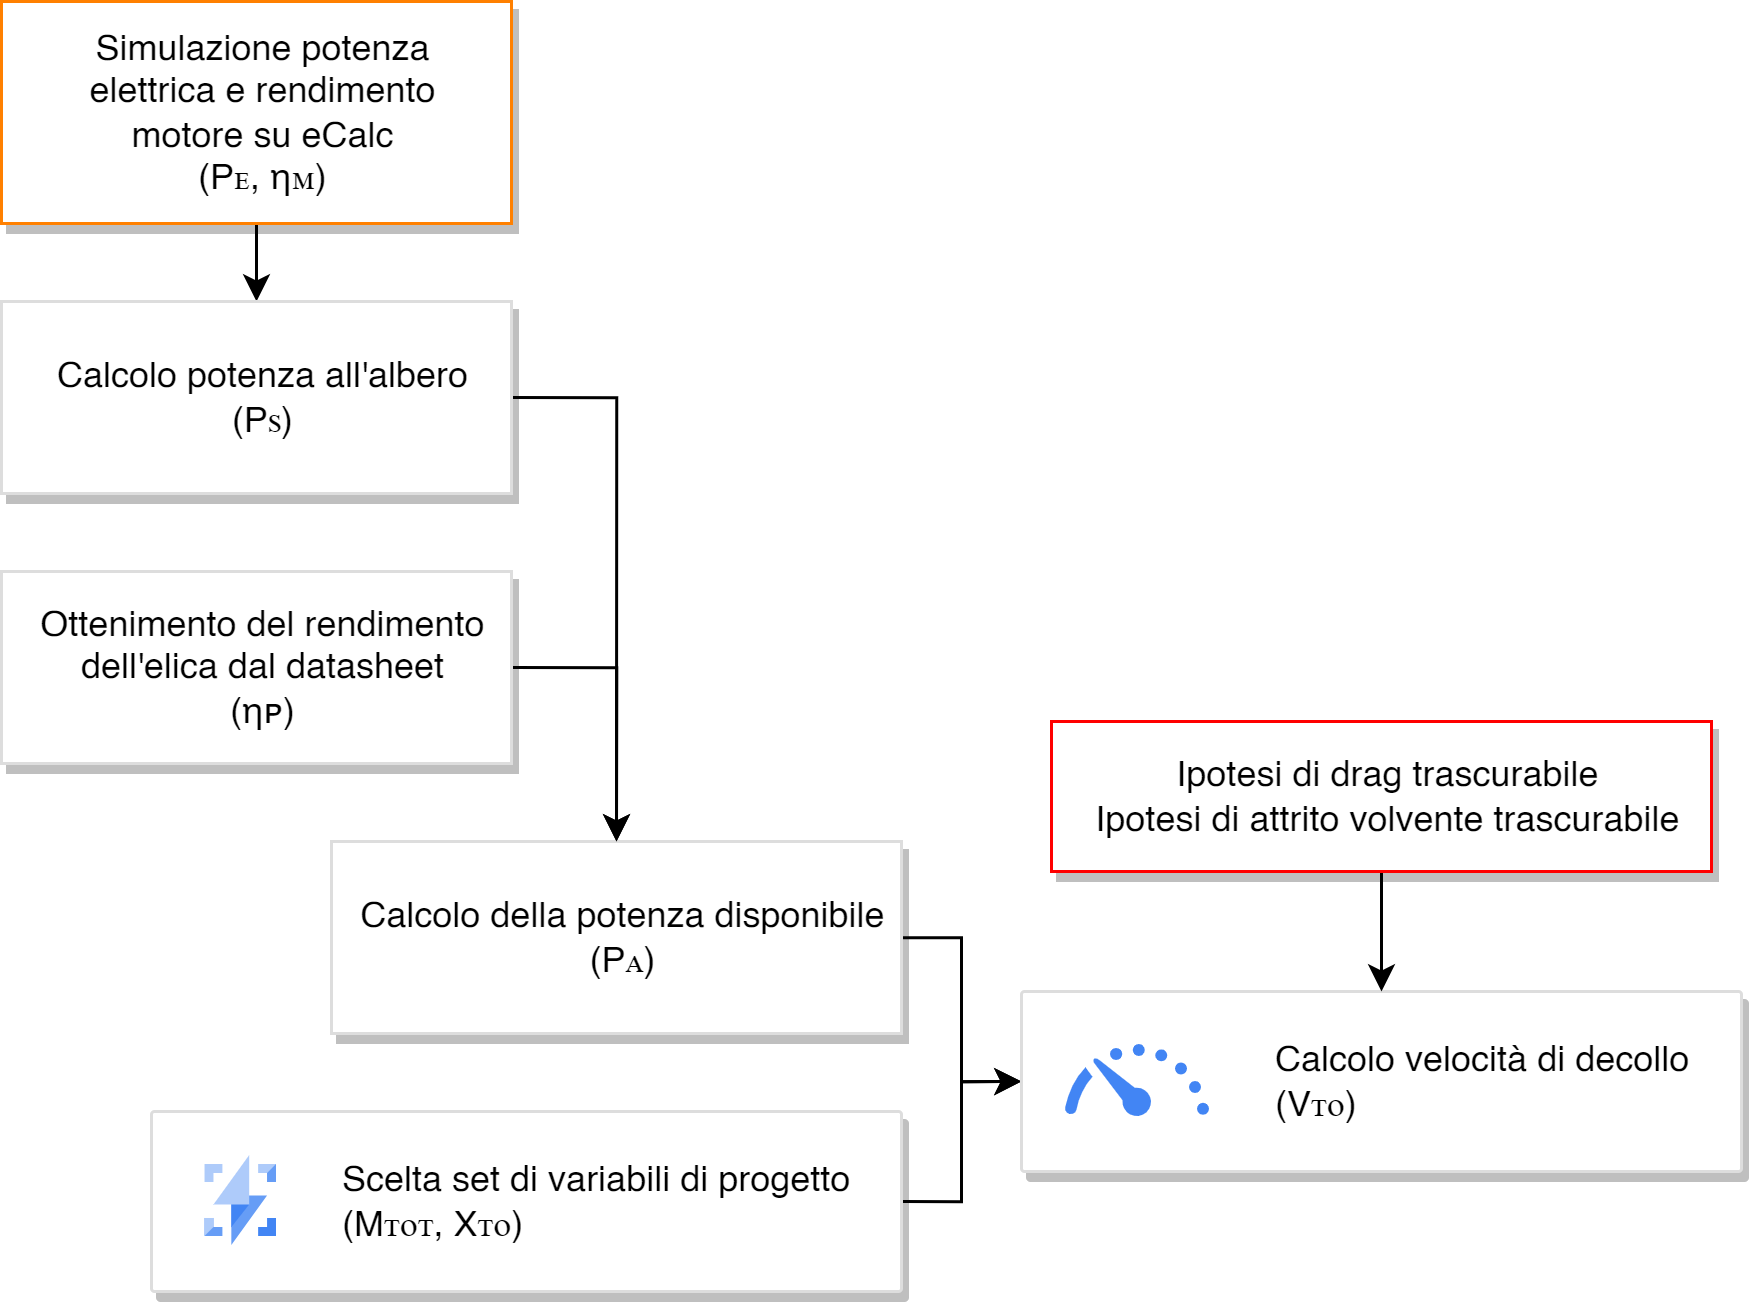
\includegraphics[width=11.6cm]{img/dim-vto-v2}
\end{figure}

\subsubsection{Verifica dei risultati di potenza propulsiva disponibile}
A seguito della competizione, sono stati resi pubblici i risultati di vari test, condotti con la stessa configurazione di elica e motore (uniformata da regolamento) in galleria del vento a throttle massimo \cite{windtunnel}. Risulta quindi utile confrontare tali dati di potenza disponibile empirici, con quelli previsti secondo modalità ed ipotesi prima descritte.

\begin{figure}[h]
	\centering
	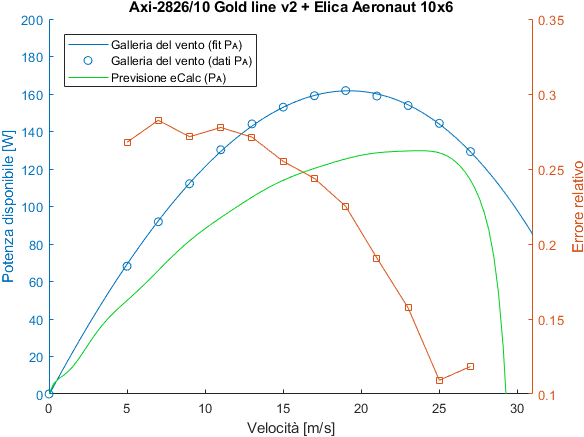
\includegraphics[width=13cm]{img/plot-PA-crop}
\end{figure}

\noindent
A tale fine è stato scritto un codice MATLAB che rappresenta il set di dati sperimentale, in termini di singoli campionamenti e con la rispettiva interpolazione polinomiale (in blu), i dati previsti (in verde) e l'errore relativo tra i due set (in rosso). 
\\\\
Si osserva che nonostante l'andamento tra le due curve di potenza sia simile, l'errore relativo nel peggiore dei casi si avvicina al 30\%. Tali risultati rimarcano l'importanza del disporre di un banco di prova delle eliche, per usare nelle future progettazioni preliminari, dati di origine empirica per correggere il modello attuale.

\subsubsection{Verifica delle ipotesi di resistenza aerodinamica e attrito volvente nulli}
Tra le ipotesi più forti utilizzate per semplificare i calcoli, ci sono quelle di resistenza aerodinamica e attrito volvente nulli. Si vuole quindi confrontare la forza considerata nel dimensionamento, ovvero la sola spinta propulsiva ($\overrightarrow{T}$), funzione della velocità, con la forza risultante realmente agente sul velivolo in fase di decollo ($\overrightarrow{R}$), anch'essa in funzione della velocità. 
\\\\
I valori di spinta propulsiva da considerare sono quelli empirici, ricavati dai test condotti in galleria del vento \cite{windtunnel}. Se infatti venissero scelti i dati previsti dal modello visto in precedenza (eCalc + datasheet elica), questi sarebbero già soggetti ai relativi errori, valutati nel paragrafo precedente, e non permetterebbero di valutare in modo isolato quelli dovuti unicamente alle ipotesi di attrito volvente e drag nulli.
\\\\
Per quanto riguarda la valutazione della forza risultante, tra i dati raccolti dal sistema di telemetria ci sono quelli di velocità rispetto al suolo, ricavati dal modulo GNSS e di accelerazione sui tre assi, provenienti dagli accelerometri. A partire da questi dati, sempre sulla base del secondo principio della dinamica, è possibile ricavare la forza risultante agente sul velivolo, che ne provoca l'accelerazione, pari alla somma vettoriale delle forze:
\begin{equation}
m \cdot \overrightarrow{a} = \overrightarrow{T} + \overrightarrow{D} + \overrightarrow{F_{AV}} = \overrightarrow{R}
\end{equation}
C'è da notare tuttavia, che la relazione precedente per come è scritta è valida solamente durante l'accelerazione orizzontale del velivolo, cioè prima che esso si stacchi da terra, in quanto a tal punto andrebbero considerate anche le componenti verticali di forze e accelerazioni.
\\\\
\noindent
A tal proposito, è stato sviluppato uno script specifico in codice Python. Tale programma in primo luogo richiede di selezionare il file .csv contenente i dati registrati durante uno specifico volo. 
\\\\
A questo punto risulta necessario isolare la porzione di dati riferita alla sola accelerazione orizzontale del velivolo. Per fare ciò si è optato per un approccio grafico: gli istanti di inizio del decollo e di liftoff possono quindi essere selezionati dall'utente direttamente sul diagramma di velocità e altitudine in funzione del tempo, e vengono evidenziati da due marker verticali (verde e rosso).
Al fine di validare la selezione, vengono visualizzati gli istanti scelti su un secondo diagramma, rappresentante le accelerazioni sui tre assi in funzione del tempo. In tale diagramma infatti, è possibile individuare l'intervallo di accelerazione orizzontale dall'osservazione qualitativa dei dati, dove appaiono ben distinguibili le vibrazioni dovute allo scorrimento del carrello sul terreno erboso.

\begin{figure}[H]
	\centering
	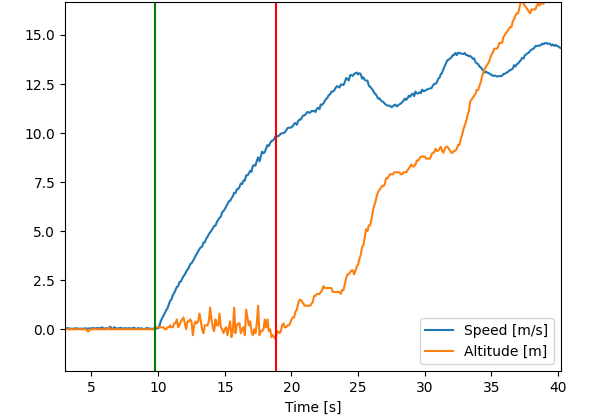
\includegraphics[width=10cm]{img/select-to-1}
\end{figure}

\vspace{-0.5cm}

\begin{figure}[H]
	\centering
	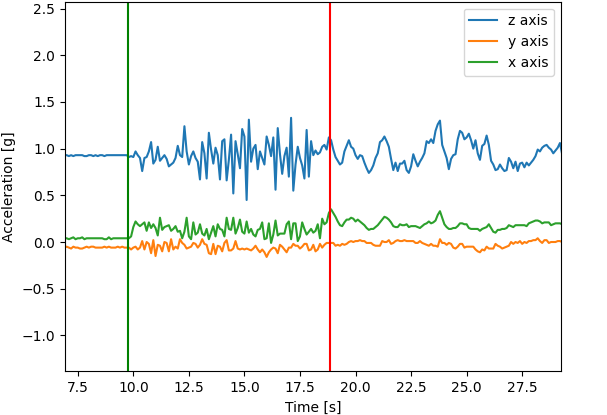
\includegraphics[width=10cm]{img/select-to-2}
	\captionsetup{labelformat=empty}
	\caption{Volo 5 - 3 luglio 2022, ore 17:51:10}
\end{figure}

\noindent
In seguito, viene richiesta in input la massa totale del velivolo al decollo, dato che è stato raccolto prima di ogni volo, e variabile in base alla quantità di payload di volta in volta stabilita.
\\\\
A questo punto il software dispone di tutti i dati necessari per calcolare l'accelerazione, e quindi la forza risultante che la provoca, al variare della velocità. Per una maggiore affidabilità dei dati, si è scelto di effettuare tale calcolo a partire da due misure indipendenti:
\begin{itemize}
\item Velocità misurata dal modulo GNSS: il dato di accelerazione viene ottenuto dal rapporto tra la variazione di velocità tra due campionamenti, e il relativo tempo intercorso: 
\begin{equation}
a_i = \frac{v_i - v_{i-1}}{t_i - t_{i-1}} = \frac{\Delta v_i}{\Delta t_i}
\end{equation}

\item Dati dell'accelerometro: in particolare quello rivolto lungo l'asse longitudinale del velivolo. 
\end{itemize}

\noindent
La forza risultante $R$ in funzione della velocità, viene quindi ottenuta dal prodotto di ognuna delle misure di accelerazione per la massa $m$, riferita al dato volo e le due linee riportate su un diagramma, insieme al valore di spinta dell'elica ($T$), che è funzione della velocità dell'aria. Si noti quindi, che il diagramma è più accurato nel caso di voli in assenza di vento, durante i quali velocità rispetto al suolo e rispetto all'aria sono praticamente coincidenti.

\begin{figure}[!h]
	\centering
	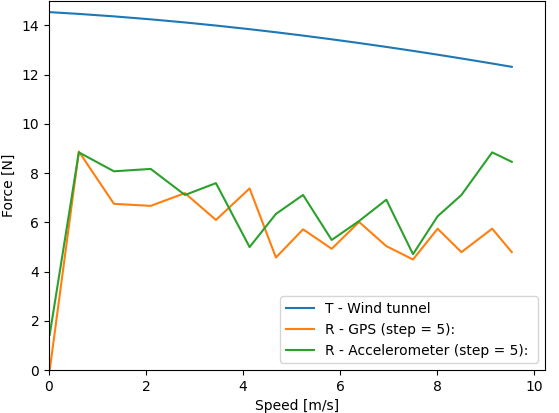
\includegraphics[width=6.5cm]{img/TvsR-6-4-c}
	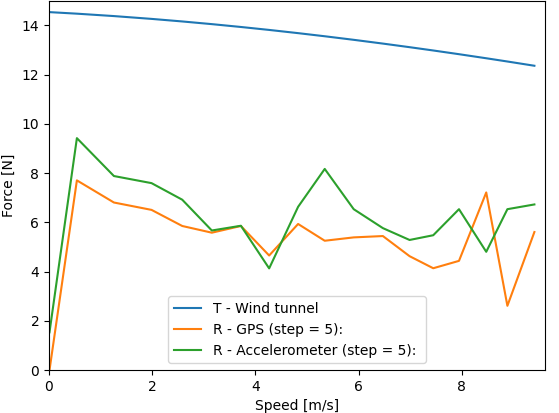
\includegraphics[width=6.5cm]{img/TvsR-6-5-c}
	\captionsetup{labelformat=empty}
	\caption{Voli 4 e 5 - 3 luglio 2022, vento assente}
\end{figure}
\begin{figure}[!h]
	\centering
	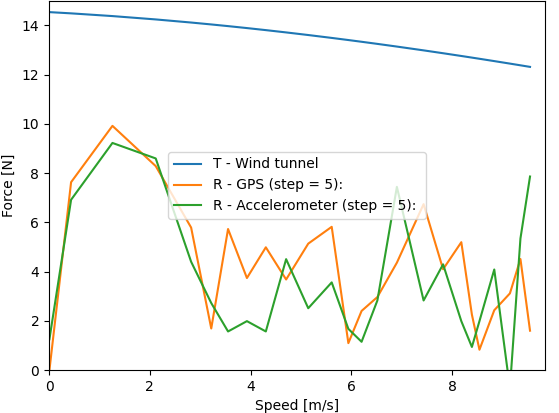
\includegraphics[width=6.5cm]{img/TvsR-7-2-c}
	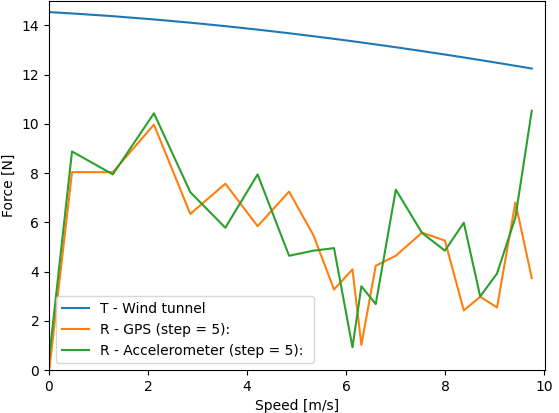
\includegraphics[width=6.5cm]{img/TvsR-7-3-c}
	\captionsetup{labelformat=empty}
	\caption{Voli 2 e 3 - 26 maggio 2023, vento assente}
\end{figure}

\noindent
A meno di alcune differenze tra un volo e l'altro, dovute a fattori quali la variazione della massa del payload caricato nella cargo-bay, l'andamento qualitativo delle linee nei vari diagrammi assume caratteristiche ricorrenti:
\begin{itemize}
\item In primo luogo le forze risultanti, calcolate sulla base delle rispettive accelerazioni al variare della velocità, hanno andamenti coerenti tra loro, a conferma del fatto che le misurazioni sono state svolte correttamente.
\item L'andamento delle forze risultanti è decrescente, con una pendenza all'incirca simile a quella della forza propulsiva.
\item Le forze risultanti, appaiono traslate verso il basso rispetto alla forza propulsiva, con valori che, punto per punto, sono intorno al 50\% di quest'ultima.
\end{itemize}
Dalle queste osservazioni quindi, si può dedurre che la differenza verticale, punto per punto, tra $T$ e $R$, rappresenta le forze resistenti di drag aerodinamico e attrito volvente del carrello che diversamente da quanto ipotizzato nel dimensionamento, non sono trascurabili.
\\\\
Possibili soluzioni da implementare per migliorare il processo di dimensionamento, potrebbero essere il quantificare tali forze resistenti, ad esempio con espressioni empiriche per stimare l'attrito volvente oppure l'adottare un processo iterativo, che in prima battuta trascuri la forza di drag per determinare una geometria di primo tentativo, e successivamente la quantifichi per affinare le geometrie dell'iterazione n-esima.

\section{Misura della velocità del flusso indisturbato}
I dati di velocità rispetto al suolo finora considerati, utilizzati per la previsione dei punteggi (sezione 3) e la verifica delle ipotesi del dimensionamento (sezione 4), sono quelli ricavati dal modulo GNSS. Nel primo caso si è trattato di una scelta forzata dagli standard imposti dal regolamento. Nel secondo caso si è scelto di utilizzare tali dati perché stabili e accurati, e in condizioni di assenza di vento, adeguati allo scopo.
\\\\
Per ulteriori valutazioni delle prestazioni tuttavia, in particolare di quelle in quota, dove non è possibile appurare l'assenza di vento, si è reso necessario disporre del dato di velocità del flusso indisturbato. Per questa ragione è stato implementato un tubo di Pitot (come da immagini a pag. 4), con le prese statica e dinamica collegate agli ingressi di un sensore di pressione differenziale. Dal dato di differenza di pressione, il sistema di telemetria a bordo ricava la velocità del flusso, secondo l'equazione di Bernoulli:

\begin{equation}
v = \sqrt{\frac{2 \cdot \Delta p}{\rho}}
\end{equation}



\newpage
\bibliography{refs}
\bibliographystyle{plain}


\end{document}